\documentclass[11pt,a4paper]{article}
\usepackage[utf8]{inputenc}
\usepackage[T1]{fontenc}
\usepackage{lmodern}
\usepackage[english]{babel}
\usepackage[margin=2.3cm]{geometry}
\usepackage{graphicx}
\usepackage{booktabs}
\usepackage{tabularx}
\usepackage{array}
\usepackage{enumitem}
\usepackage{textcomp}
\usepackage{xcolor}
\usepackage{microtype}
\usepackage[hidelinks]{hyperref}
\graphicspath{{images/}{enclosure/out/}}
\setlist{itemsep=2pt, topsep=4pt}
\newcolumntype{L}{>{\raggedright\arraybackslash}X}
\renewcommand{\arraystretch}{1.15}

\title{MP3 Player\\[4pt]\large A hi-fi music player with a retro look}
\author{Stefan Jipa}
\date{\today}

\begin{document}
\maketitle

\begin{center}
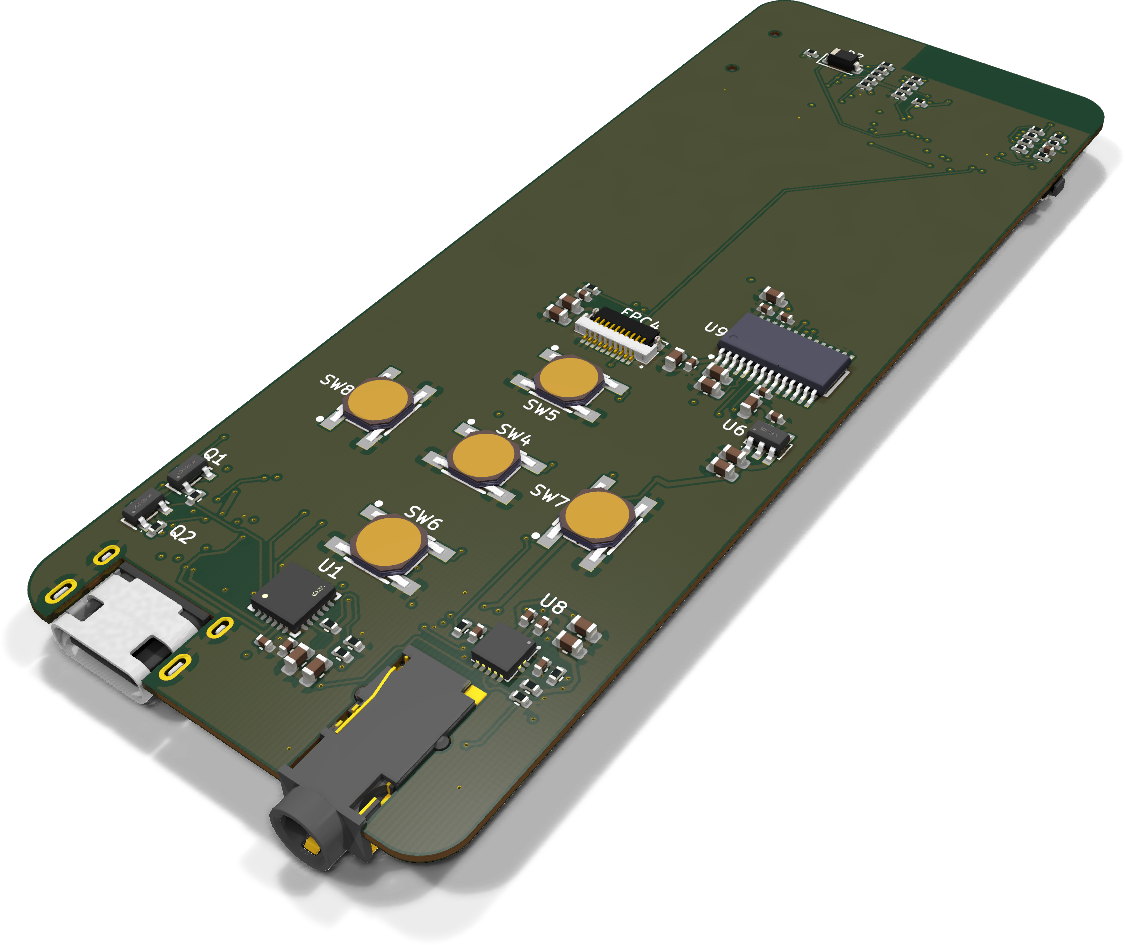
\includegraphics[width=0.46\textwidth]{pcb_iso.png}
\end{center}

\tableofcontents
\newpage

\section{Goal}
Build a good, modern MP3 player with a retro style, going all out on the design.
It plays FLAC/WAV through a proper DAC and headphone amplifier, streams to Bluetooth headphones,
and has a reflective display that stays readable in direct sunlight.

\section{Requirements}
\begin{itemize}
  \item Custom PCB designed in KiCad, assembled by JLCPCB with as many parts as possible from their stock.
  \item Compact: target case $41 \times 102 \times 8$\,mm.
  \item Highest possible audio quality on the 3.5\,mm jack (FLAC/WAV, not just MP3).
  \item Bluetooth A2DP to wireless headphones.
  \item 3.5\,mm jack with plug detection.
  \item Push-push microSD card.
  \item USB-C for charging and programming (USB-UART), with ESD protection.
  \item Thin single-cell LiPo with charger, fuel gauge and soft power (power on from a button).
  \item Battery safety: only cells with a built-in protection circuit, charge current limited to 0.5\,C, firmware cut-off at $V_\mathrm{BAT} \approx 3.4$\,V.
  \item Display readable in sunlight.
  \item v1 without speakers (WM8960 or a class-D amplifier stay for v2).
\end{itemize}

\section{Architecture}
\begin{small}
\begin{verbatim}
USB-C - ESD -+- CP2102N -- auto-reset -- ESP32-PICO-MINI-02
             +- BQ25180 (charger + power path + ship mode + button)
                  | VSYS
                  +- TPS63802 buck-boost -- 3.3 V digital (ESP32, SD, display)
                  +- LP5907 LDO ---------- clean 3.3 V analog (DAC)
                  +- LM27762 ------------- clean +/-3 V rails (headphone amp)
                LiPo -- MAX17048 (fuel gauge, I2C)

ESP32 -- I2S -- PCM5122 (DAC) -- OPA1622 (headphone amp) -- 3.5 mm jack
      +- SDMMC 4-bit -- microSD push-push
      +- SPI -- Sharp LS013B7DH03 memory LCD
      +- I2C -- BQ25180, MAX17048, PCM5122
      +- GPIO -- click wheel, buttons, jack and card detect
      +- BT A2DP -- wireless headphones
\end{verbatim}
\end{small}

Only the classic ESP32 has Bluetooth Classic (A2DP); the S3, C3 and C6 are BLE only.
The ESP32-PICO-MINI-02 module brings 8\,MB flash, 2\,MB PSRAM for audio buffers, and a certified antenna.

\section{Components}
\begin{table}[h]
\centering\small
\begin{tabularx}{\textwidth}{@{}lL l@{}}
\toprule
Block & Part & LCSC \\
\midrule
MCU & ESP32-PICO-MINI-02-N8R2 & C2980306 \\
DAC & PCM5122PW, 112\,dB, 32-bit/384\,kHz, volume over I2C & C1540085 \\
Headphone amp & OPA1622, VSON-10 & C2876559 \\
Amp rails & LM27762, $\pm$ charge pump + LDOs & C473398 \\
Jack & PJ-342C CB, 4-pole, sinking, with HP-DET & C49287245 \\
Charger & BQ25180, I2C, power path, ship mode + button & C3682423 \\
3.3\,V digital & TPS63802 buck-boost, 2\,A, with 0.47\,\textmu H WPN201610 & C2845237 \\
3.3\,V analog & LP5907-3.3 low-noise LDO & C80670 \\
Fuel gauge & MAX17048 & C2682616 \\
USB-C & TYPE-C 16P CB0.8, sinking, for 0.8\,mm boards & C2906289 \\
USB-UART & CP2102N-A02-GQFN24 (QFN-24 has DTR for auto-reset) & C969151 \\
ESD & USBLC6-2SC6 on D+/D$-$ & C7519 \\
microSD & TF-01A push-push & C91145 \\
Display & Sharp LS013B7DH03 1.28'' $128\times128$ memory LCD & (DigiKey/Mouser) \\
Display FPC & Hirose FH19C-10S, 0.9\,mm tall & C598004 \\
Buttons & TS-1187B-B (wheel, $\times5$), EVQP7J01P (power), TS-1088 (EN/BOOT) & C500066 \dots \\
Battery & LiPo LP403759, 1000\,mAh, $4\times37\times59$\,mm, JST SH & C160402 (conn.) \\
\bottomrule
\end{tabularx}
\end{table}

Passives are chosen for quality: 0.1\,\% thin-film resistors in the audio path and the rail dividers,
C0G capacitors in the DAC output filter, and bulk capacitors in 0603/0805 so they keep their value under DC bias.
Every part carries its LCSC code in the \texttt{LCSC Part} field, which feeds the JLC BOM.
The full table with stock and prices is in \texttt{mp3\_player.md}.

\section{Power}
\begin{itemize}
  \item \textbf{Soft power.} A press of the button brings the BQ25180 out of ship mode; the ESP32 turns the player off by sending the ship-mode command over I2C, after which the battery draws only a few nA. A long press is a hardware reset.
  \item \textbf{Rails.} VSYS from the charger's power path feeds three regulators: the TPS63802 buck-boost for the digital 3.3\,V (it can drain the cell fully and handles Bluetooth/WiFi peaks), the LP5907 for a clean analog 3.3\,V for the DAC, and the LM27762 for $\pm3$\,V around the headphone amplifier.
  \item \textbf{Charging.} 0.5\,C, i.e.\ 500\,mA for the 1000\,mAh cell, about 2.5\,h. Estimated runtime is 11--13\,h on the jack and 7--8\,h on Bluetooth.
\end{itemize}

\section{Audio}
The ESP32 sends I2S to the PCM5122, which runs from its internal PLL (no MCLK) and sets the volume in hardware.
An RC filter with C0G capacitors feeds the OPA1622, powered from the LM27762's clean $\pm$ rails, which drives the jack directly.
Plug detection comes from the jack's HP-DET contact. Bluetooth audio is limited by SBC, since the ESP32 has no aptX or LDAC.

Layout rules for the audio path: one solid ground plane with no split (as TI recommends for the PCM512x),
the DAC and amplifier far from the ESP32 and the buck-boost inductor, and no fast digital trace next to the analog nets.
The OPA1622's exposed pad is V$-$ ($-3$\,V), not ground.

\section{PCB}
\begin{center}
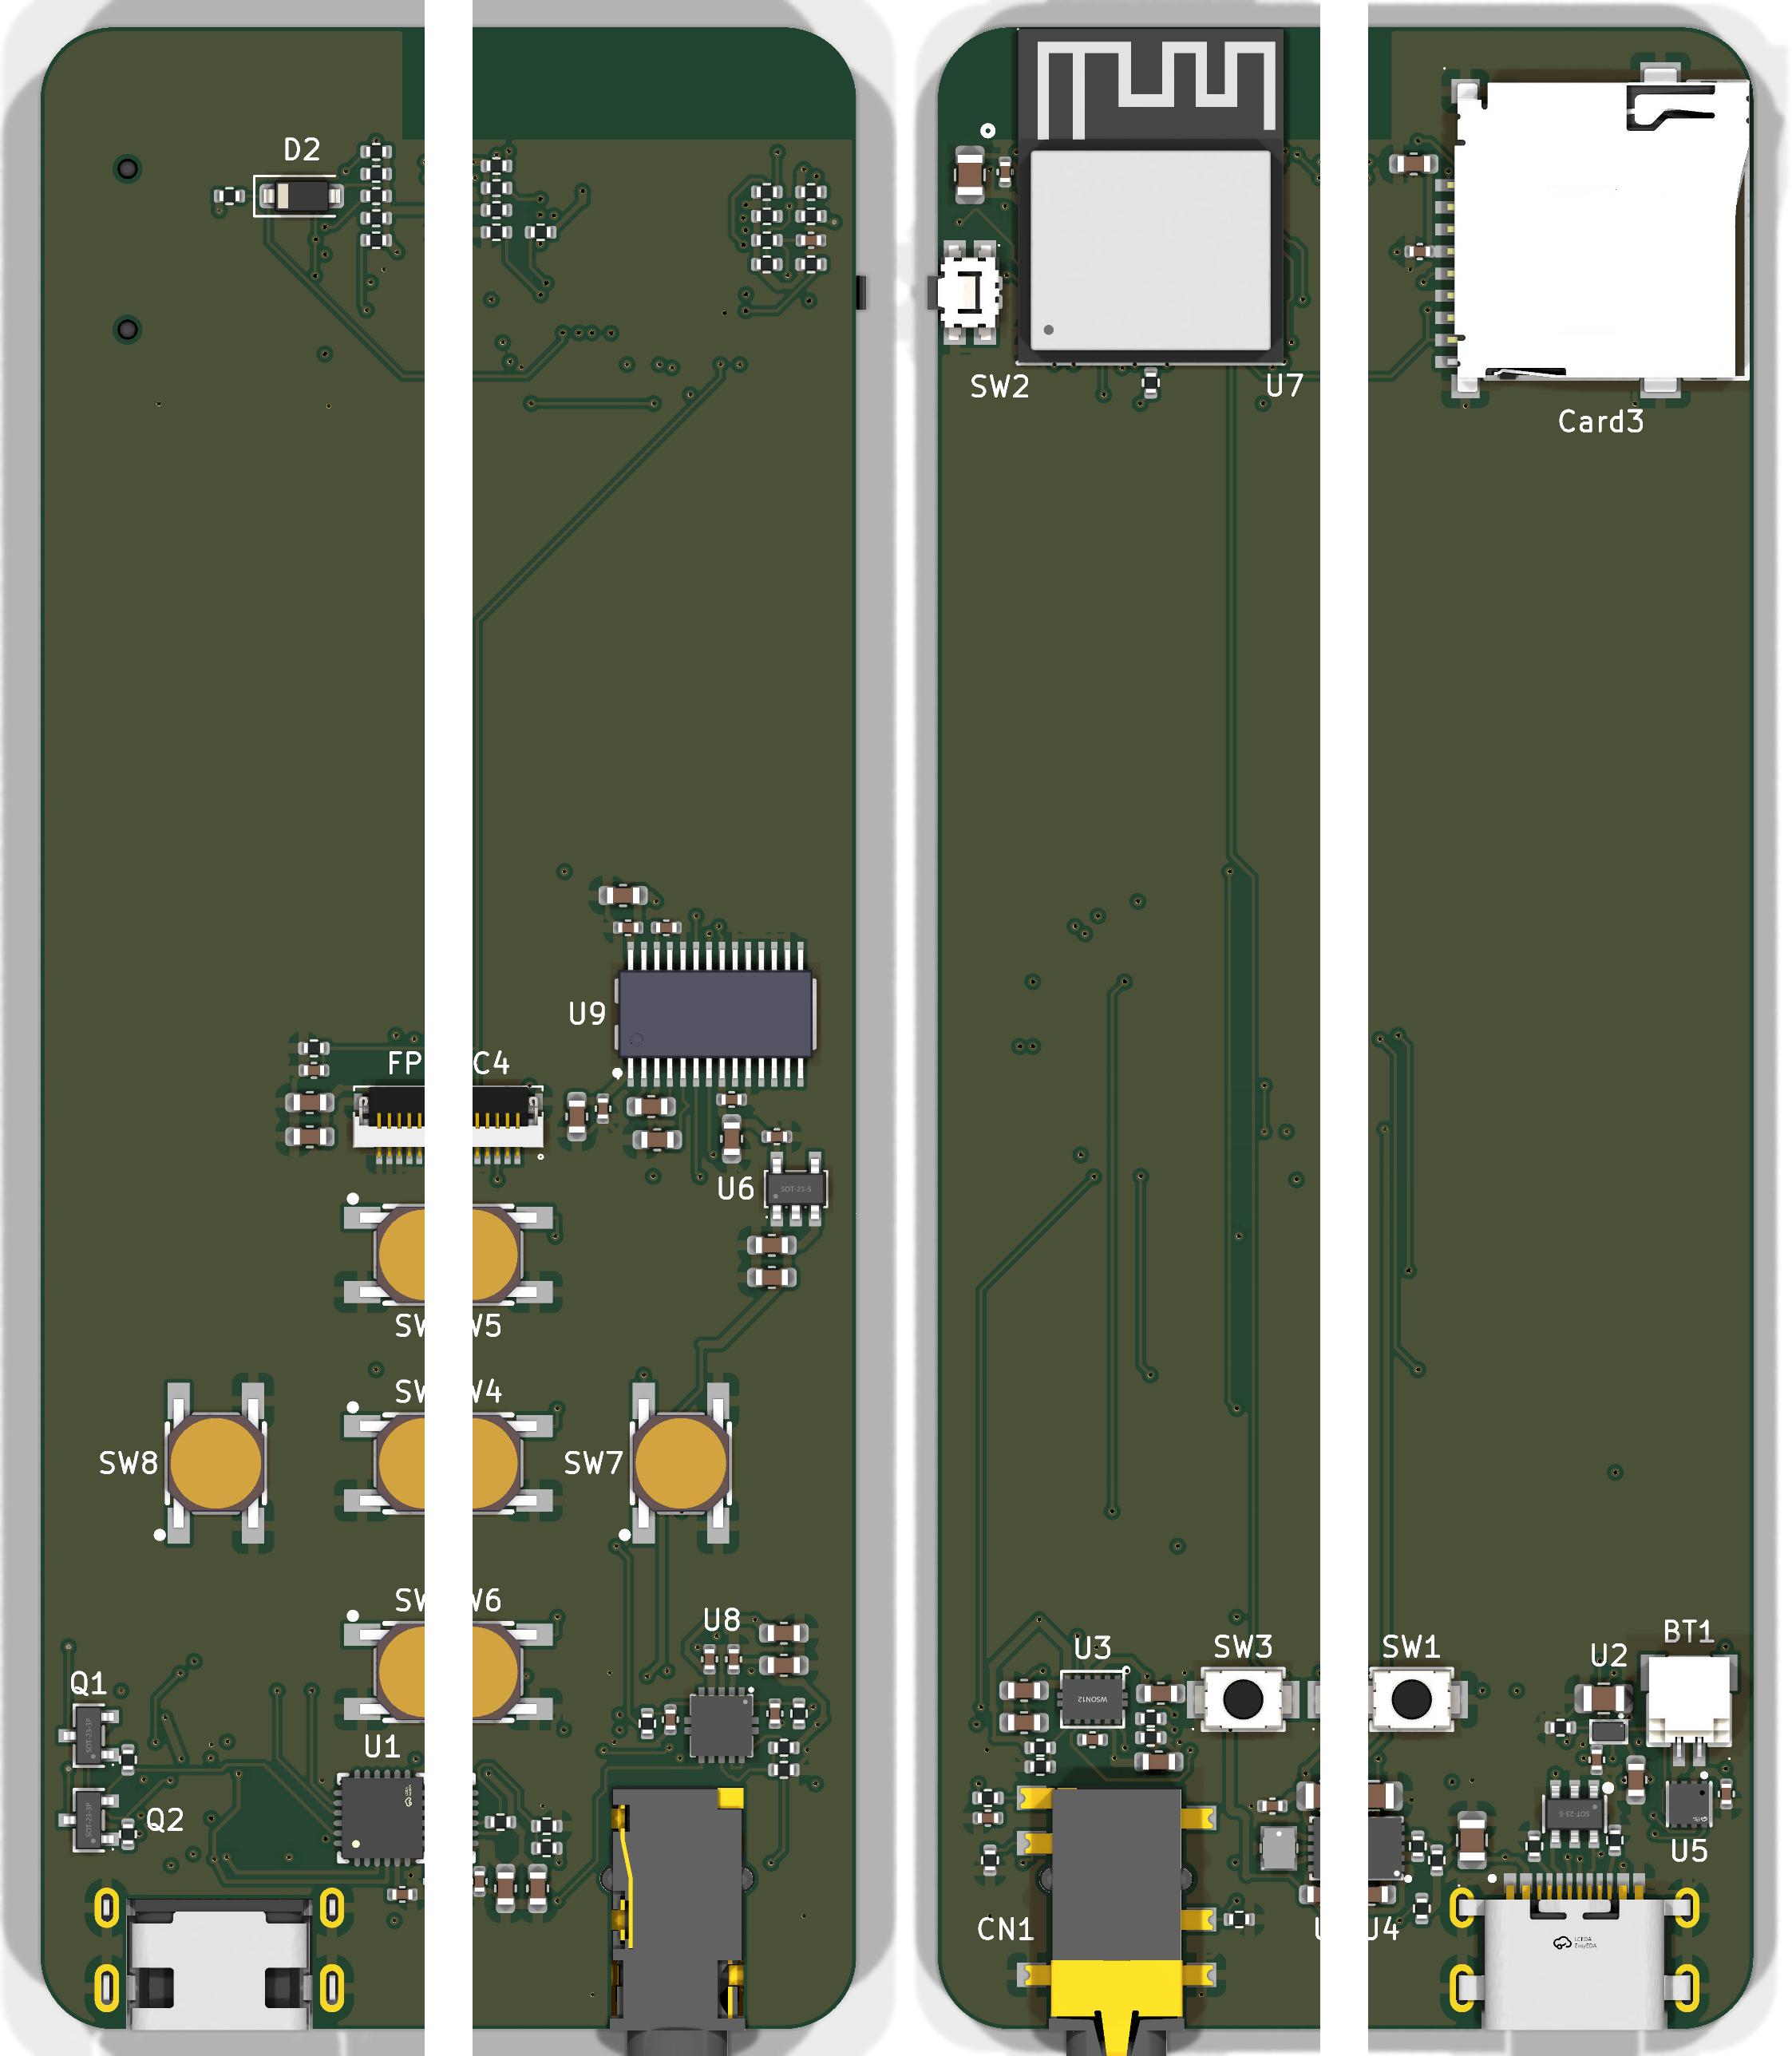
\includegraphics[width=0.55\textwidth]{pcb_front_back.png}\\[2pt]
{\small Front (left) and back (right).}
\end{center}

\begin{itemize}
  \item \textbf{Stackup.} 4 layers, 0.8\,mm, ENIG: signals on Front, a solid GND plane on In1, signals and GND pour on In2, signals on Back. Outline $38.2 \times 99.6$\,mm with R3.6 corners, taken from the enclosure model.
  \item \textbf{Rules.} 0.15\,mm track and clearance, 0.45/0.2\,mm vias (JLC's smallest via without surcharge), power nets at 0.3--0.4\,mm.
  \item \textbf{Placement.} The front carries only low parts: display connector, click-wheel switches, DAC, amplifier, USB-UART. The back has the ESP32 and microSD at the top, the battery over the middle, and the charger, fuel gauge, buck-boost and $\pm$ rails in the bottom strip between the sinking USB-C and the jack. The ESP32 antenna sits at the top edge with no copper under it.
  \item \textbf{Routing.} The buck-boost loop, the USB-C data pair and CC lines, the BQ25180 ball escapes and the amplifier rails were routed by hand; the rest with Freerouting. Ground pours on Front, Back and In2 with stitching vias.
  \item \textbf{Checks.} DRC: 0 errors, 0 unconnected items. ERC: 0. No fast digital net comes within 1\,mm of the audio traces.
\end{itemize}

\section{Enclosure}
\begin{center}
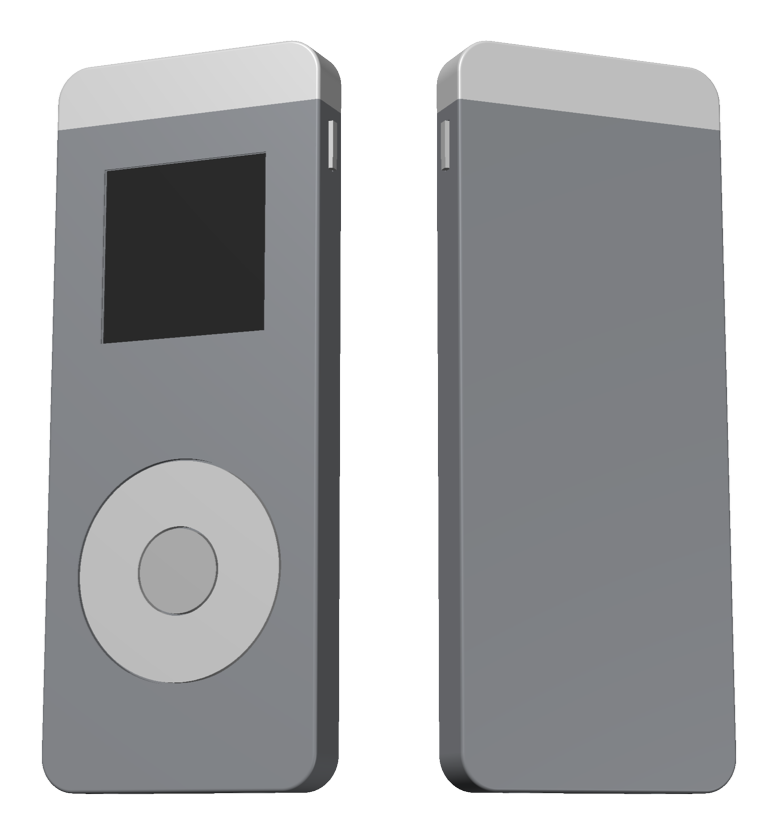
\includegraphics[width=0.5\textwidth]{hero_B.png}
\end{center}
A vertical, iPod-style case, $41 \times 102.4 \times 8.0$\,mm, CNC-machined from anodized 6061 aluminium for v1 (titanium for v2).
The display sits at the top of the front face behind a clear window, with the click wheel below it: a 3D-printed ring
rocking on four switches plus a centre play button. Since a metal shell blocks the radio, the top 9\,mm is a printed plastic cap with
the ESP32 antenna right under it. The back is flat. USB-C and the jack sit on the bottom face; the case thickness is set
so the 6\,mm jack hole stays on the flat part of the bottom face. The model is parametric, written with build123d in \texttt{enclosure/concept.py}.

\section{Assembly and cost}
JLC assembles only the parts that cannot be soldered by hand (QFN, DFN, BGA, LGA) plus the passives. Connectors,
buttons, the LP5907 and the USBLC6 come in the same LCSC order and are soldered at home: USB-C and microSD first,
then the FPC, then the jack, buttons and battery.

Because parts sit on both sides, the board needs JLC's Standard assembly. The estimate from 19 November 2026 is about \$200
for two assembled boards out of five PCBs, including VAT. Two parts were out of stock that day (PCM5122, and the 511\,k$\Omega$ feedback resistor);
drop-in replacements are noted in \texttt{mp3\_player.md}, and stock is re-checked before ordering.

\section{Firmware}
\sloppy
ESP-IDF or Arduino with \texttt{arduino-audio-tools} and \texttt{ESP32-A2DP}: read the card, decode MP3/FLAC, and send it to I2S (jack) or A2DP (Bluetooth).
Hardware limits the firmware must respect:
\begin{itemize}\sloppy
  \item Burn the eFuse once per board before the first flash, because SD D2 sits on the GPIO12 strapping pin:\\ \texttt{espefuse.py set\_flash\_voltage 3.3V}
  \item Keep the PCM5122 digital volume at or below about $-4$\,dB: the OPA1622 runs on $\pm3$\,V and clips above about 1.5\,Vrms.
  \item Shut down at $V_\mathrm{BAT} \approx 3.4$\,V, below which the LP5907 drops out.
  \item Set the BQ25180 charge current over I2C at every boot (it starts at about 10\,mA).
  \item Before ship mode, set the MAX17048 to sleep so it draws under 1\,\textmu A.
  \item Clear the display memory before raising \texttt{LCD\_DISP}, and toggle VCOM about once a second.
\end{itemize}

\section{Tests}
Planned bring-up, in order:
\begin{enumerate}
  \item Bare board: continuity VBUS--GND, VBAT--GND, D+/D$-$ to the CP2102N, no shorts on any rail.
  \item USB power without a battery: VSYS, 3.3\,V digital, 3.3\,V analog; $\pm3$\,V with \texttt{AUDIO\_EN} high.
  \item Programming: auto-reset into download mode, eFuse, first flash.
  \item Battery: correct polarity on the JST connector, charge current at 500\,mA, charging stops at full, cell temperature stays near ambient while charging.
  \item Ship mode: current from the battery in ship mode, wake from the button.
  \item Fuel gauge: voltage and state of charge read over I2C, cut-off at 3.4\,V.
  \item Audio: sine at $-4$\,dBFS into 32\,$\Omega$ without clipping, noise floor with no signal, jack detect.
  \item Storage and display: SD in 4-bit mode, card detect, display clear and VCOM.
  \item Bluetooth A2DP to headphones; WiFi upload.
\end{enumerate}

\section{Resources}
\begin{itemize}
  \item Datasheets for every part in \texttt{datasheets/}, including the ESP32 hardware design guidelines.
  \item Pin-by-pin schematic connections: \texttt{connections.md}.
  \item Project documentation and status: \texttt{mp3\_player.md}.
  \item JLC parts: \url{https://jlcpcb.com/parts}
  \item arduino-audio-tools: \url{https://github.com/pschatzmann/arduino-audio-tools}
  \item ESP32-A2DP: \url{https://github.com/pschatzmann/ESP32-A2DP}
  \item Repository: \url{https://github.com/stefanVanadium/mp3-player}
\end{itemize}

\end{document}
